% A LaTeX (non-official) template for ISAE projects reports
% Copyright (C) 2014 Damien Roque
% Version: 0.2
% Author: Damien Roque <damien.roque_AT_isae.fr>

\documentclass[a4paper,12pt]{book}
\usepackage[utf8]{inputenc}             % The input file is in utf-8
\usepackage{marvosym}                   % This package provides some symbols. The € is 
\DeclareUnicodeCharacter{20AC}{\EUR{}} 
\usepackage{textcomp}
\usepackage[T1]{fontenc}
\usepackage[frenchb]{babel} % If you write in French
%\usepackage[english]{babel} % If you write in English
\usepackage{a4wide}
\usepackage{graphicx}
\usepackage{lmodern}
\usepackage{amsmath}
\usepackage{amssymb}
\usepackage{mathrsfs}
\usepackage{xcolor}
\usepackage{sectsty}

\usepackage{titlesec}
\definecolor{MyBlue}{RGB}{29, 82, 119}
\definecolor{Orange}{RGB}{209, 113, 0}
\sectionfont{\color{MyBlue}}  % sets colour of sections


\setcounter{secnumdepth}{4}

\usepackage{titlesec}
\titleformat*{\section}{\Large\bfseries\sffamily}
\titleformat*{\subsection}{\large\bfseries\sffamily}
\titleformat*{\subsubsection}{\bfseries\sffamily\color{MyBlue}}



\graphicspath{{images/}}
\usepackage{subfig}
\usepackage{tikz}
\usepackage{float} 
\usetikzlibrary{shapes,arrows}
\usepackage{pgfplots}
\pgfplotsset{compat=newest}
\pgfplotsset{plot coordinates/math parser=false}
\newlength\figureheight
\newlength\figurewidth
\pgfkeys{/pgf/number format/.cd,
set decimal separator={,\!},
1000 sep={\,},
}
\usepackage{ifthen}
\usepackage{ifpdf}
\ifpdf
\usepackage[pdftex]{hyperref}
\else
\usepackage{hyperref}
\fi
\usepackage{color}
\hypersetup{%
colorlinks=true,
linkcolor=black,
citecolor=black,
urlcolor=black}

\renewcommand{\baselinestretch}{1.05}
\usepackage{fancyhdr}
\pagestyle{fancy}
\fancyfoot{}
\fancyhead[LE,RO]{\bfseries\thepage}
\fancyhead[RE]{\bfseries\nouppercase{\leftmark}}
\fancyhead[LO]{\bfseries\nouppercase{\rightmark}}
\setlength{\headheight}{15pt}

\let\headruleORIG\headrule
\renewcommand{\headrule}{\color{black} \headruleORIG}
\renewcommand{\headrulewidth}{1.0pt}
\usepackage{colortbl}
\arrayrulecolor{black}

\fancypagestyle{plain}{
  \fancyhead{}
  \fancyfoot[C]{\thepage}
  \renewcommand{\headrulewidth}{0pt}
}

\makeatletter
\def\@textbottom{\vskip \z@ \@plus 1pt}
\let\@texttop\relax
\makeatother

\makeatletter
\def\cleardoublepage{\clearpage\if@twoside \ifodd\c@page\else%
  \hbox{}%
  \thispagestyle{empty}%
  \newpage%
  \if@twocolumn\hbox{}\newpage\fi\fi\fi}
\makeatother

\usepackage{amsthm}
\usepackage{amssymb,amsmath,bbm}
\usepackage{array}
\usepackage{bm}
\usepackage{multirow}
\usepackage[footnote]{acronym}

\newcommand*{\SET}[1]  {\ensuremath{\mathbf{#1}}}
\newcommand*{\VEC}[1]  {\ensuremath{\boldsymbol{#1}}}
\newcommand*{\FAM}[1]  {\ensuremath{\boldsymbol{#1}}}
\newcommand*{\MAT}[1]  {\ensuremath{\boldsymbol{#1}}}
\newcommand*{\OP}[1]  {\ensuremath{\mathrm{#1}}}
\newcommand*{\NORM}[1]  {\ensuremath{\left\|#1\right\|}}
\newcommand*{\DPR}[2]  {\ensuremath{\left \langle #1,#2 \right \rangle}}
\newcommand*{\calbf}[1]  {\ensuremath{\boldsymbol{\mathcal{#1}}}}
\newcommand*{\shift}[1]  {\ensuremath{\boldsymbol{#1}}}

\newcommand{\eqdef}{\stackrel{\mathrm{def}}{=}}
\newcommand{\argmax}{\operatornamewithlimits{argmax}}
\newcommand{\argmin}{\operatornamewithlimits{argmin}}
\newcommand{\ud}{\, \mathrm{d}}
\newcommand{\vect}{\text{Vect}}
\newcommand{\sinc}{\ensuremath{\mathrm{sinc}}}
\newcommand{\esp}{\ensuremath{\mathbb{E}}}
\newcommand{\hilbert}{\ensuremath{\mathcal{H}}}
\newcommand{\fourier}{\ensuremath{\mathcal{F}}}
\newcommand{\sgn}{\text{sgn}}
\newcommand{\intTT}{\int_{-T}^{T}}
\newcommand{\intT}{\int_{-\frac{T}{2}}^{\frac{T}{2}}}
\newcommand{\intinf}{\int_{-\infty}^{+\infty}}
\newcommand{\Sh}{\ensuremath{\boldsymbol{S}}}
\newcommand{\C}{\SET{C}}
\newcommand{\R}{\SET{R}}
\newcommand{\Z}{\SET{Z}}
\newcommand{\N}{\SET{N}}
\newcommand{\K}{\SET{K}}
\newcommand{\reel}{\mathcal{R}}
\newcommand{\imag}{\mathcal{I}}
\newcommand{\cmnr}{c_{m,n}^\reel}
\newcommand{\cmni}{c_{m,n}^\imag}
\newcommand{\cnr}{c_{n}^\reel}
\newcommand{\cni}{c_{n}^\imag}
\newcommand{\tproto}{g}
\newcommand{\rproto}{\check{g}}
\newcommand{\LR}{\mathcal{L}_2(\SET{R})}
\newcommand{\LZ}{\ell_2(\SET{Z})}
\newcommand{\LZI}[1]{\ell_2(\SET{#1})}
\newcommand{\LZZ}{\ell_2(\SET{Z}^2)}
\newcommand{\diag}{\operatorname{diag}}
\newcommand{\noise}{z}
\newcommand{\Noise}{Z}
\newcommand{\filtnoise}{\zeta}
\newcommand{\tp}{g}
\newcommand{\rp}{\check{g}}
\newcommand{\TP}{G}
\newcommand{\RP}{\check{G}}
\newcommand{\dmin}{d_{\mathrm{min}}}
\newcommand{\Dmin}{D_{\mathrm{min}}}
\newcommand{\Image}{\ensuremath{\text{Im}}}
\newcommand{\Span}{\ensuremath{\text{Span}}}

\newtheoremstyle{break}
  {11pt}{11pt}%
  {\itshape}{}%
  {\bfseries}{}%
  {\newline}{}%
\theoremstyle{break}

%\theoremstyle{definition}
\newtheorem{definition}{Définition}[chapter]

%\theoremstyle{definition}
\newtheorem{theoreme}{Théorème}[chapter]

%\theoremstyle{remark}
\newtheorem{remarque}{Remarque}[chapter]

%\theoremstyle{plain}
\newtheorem{propriete}{Propriété}[chapter]
\newtheorem{exemple}{Exemple}[chapter]

\parskip=5pt
%\sloppy

\begin{document}
\let\cleardoublepage\clearpage
%%%%%%%%%%%%%%%%%%
%%% First page %%%
%%%%%%%%%%%%%%%%%%


\begin{titlepage}
\begin{center}

\includegraphics[width=0.6\textwidth]{images/univ.png}

\vfill

{\large Université de Paris Ouest Nanterre La Défense}\\[0.7cm]

{\large Mémoire Master 2 MIAGE}\\[0.7cm]



% Title
\rule{\linewidth}{0.5mm} \\[0.4cm]
{ \huge \bfseries Prédiction de la stratégie de récupération d'un service Web composite\\[0.4cm] }
\rule{\linewidth}{0.5mm} \\[1.5cm]

\vfill
\vfill
\vfill

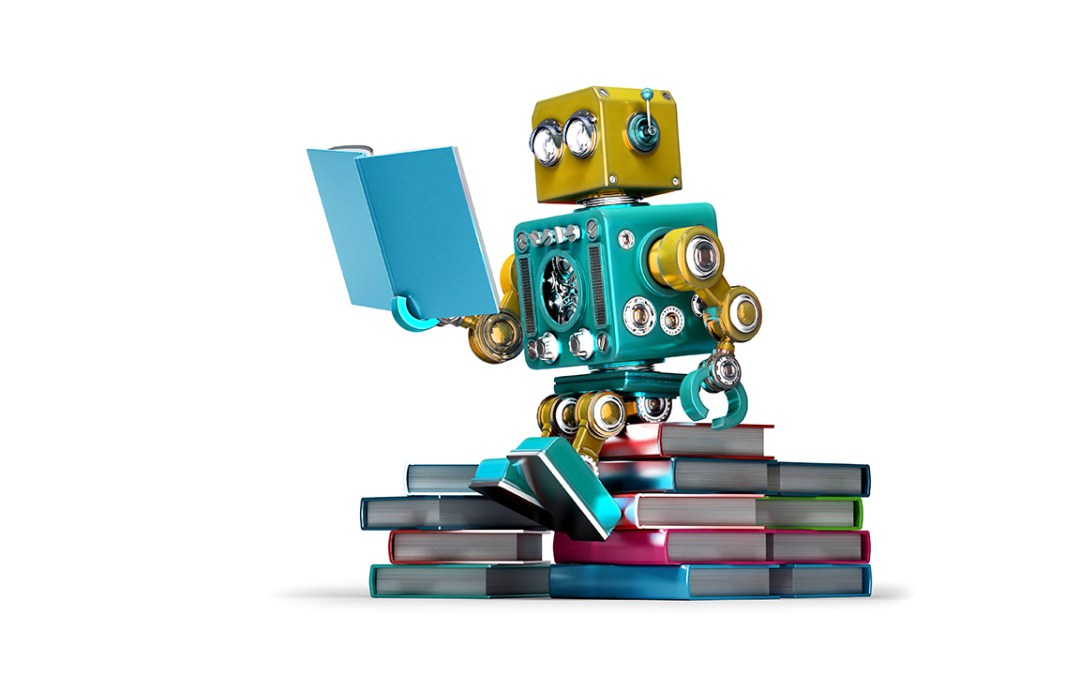
\includegraphics[width=0.6\textwidth]{images/ML.jpg}


% Author and supervisor
\noindent
\begin{minipage}{0.7\textwidth}
  \large
    \emph{Réalisé par :}\\
- Nadia \textsc{MASLOUHI}\\
\end{minipage}%
\begin{minipage}{0.7\textwidth}
   \large
    \emph{Encadré par :} \\
- Mme.~Castillo Marta \textsc{RUKOZ}
\end{minipage}

\vfill
\vfill
\vfill
\vfill
\vfill
\vfill
% Bottom of the page
\large{ 18 juin 2018}


\end{center}
\end{titlepage}
\clearpage

\chapter*{Remerciements}

Je tiens en premier lieu à remercier Mme Castillo Marta RUKOZ mon encadrante pédagogique pour sa proposition de sujet de mémoire d'une part, et pour son suivi durant la période de réalisation d'autre part.

J'aimerais également remercier tous les professeurs qui m'ont enseigné et qui m'ont aidé a travers leurs conseils pour l'amélioration de ce travail.

Je tiens à remercier vivement Hassan MASLOUHI, mes parent et toutes ma famille et mes amis qui m’ont soutenue et m’ont encouragée durant toute l'année.

Enfin, je souhaite remercier Mr Christophe PHILIPPE pour son encouragement, et son soutien en m'offrant le temps pour la rédaction du mémoire.



\chapter*{Résumé}

Dans ce mémoire, nous présentons une approche de prédiction pour les services Web composites,
qui permet de prédire le mécanisme de récupération en cas de défaillance d'un service Web composant.
Notre étude se base sur une approche d'exécution auto-corrective (self-healing) de services Web composites, qui se base sur des agents qui sont capables de prendre, d'une manière automatique, des décisions pendant l'exécution des services, à partir de leurs connaissances et la base d'informations qu'ils ont.
les agents font des déductions, en fonction des informations qu'ils ont sur le service, sur eux-même, en prenant en compte ce qui est attendu et ce qui se passe réellement lors de l'exécution.

Notre contribution dans ce mémoire consiste la restitution de toute cette base d'informations, ainsi que les stratégies de récupérations sélectionnées après la fin d'exécution, pour les exploiter comme des données  d'apprentissage automatique. 

Les algorithmes de classification de Machine Learning nous ont permet de construire des modèles qui permettent de prédire le mécanisme de récupération en cas de panne sur les services composites.

La collecte et le traitement des données sont faits a travers l'outil Pentaho Data Integration, qui offre une extension de Machine Learning a travers WEKA, dans laquelle on a exécuté tous les algorithmes de classification en mesurant leurs performances de précision.

\textbf{Mots clés : Service Web Composite, Tolérance aux pannes, stratégie de récupération, Machine Learning, Classification }


\tableofcontents
\listoffigures
%%%%%%%%%%%%%%%%%%%%%%%%%%%%%%%%%%%%%%%%%%%%
%%% Content of the report and references %%%
%%%%%%%%%%%%%%%%%%%%%%%%%%%%%%%%%%%%%%%%%%%%

\mainmatter
\pagestyle{fancy}





\title{La mise en place d'un générateur du code automatique d’après une Modélisation DOMIS}

\author{nadia.maslouhi }


\section{Introduction}

\vspace{1cm}
B-ADSC (Bucki – Analyse décisionnelle des Systèmes complexes )  est une méthode dédiée à la conception et à l’analyse des systèmes et des organisations qui se base sur l’approche décisionnelle.

L'approche décisionnelle des systèmes complexes consiste en la conception, l'analyse et l'optimisation d'une organisation de telle sorte que les savoir-faire et les procédés employés puissent s’exprimer avec le plus d'efficacité et en totale convergence de buts avec la finalité de l'ensemble.

\vspace{0,5cm}

L'analyse décisionnelle des systèmes complexes met l'accent sur la capacité des organisations pour prendre des décisions sur le pilotage des processus. 
Cet conception se base principalement sur la fixation du but principal et l’élaboration des décisions d’une manière intelligente tout en contrôlant leur évolution afin de les amener à une situation en accord avec l’objectif initial.

\vspace{0,5cm}

Pour B-ADSC, une organisation correspond à une hiérarchie opérationnelle d’activités dans laquelle chaque activité représente « un centre élémentaire de prise de décision » pouvant être piloté par un homme ou par une machine.

Une activité est chargée du pilotage (régulation) du processus en fonction des objectifs qui lui sont assignés par l'environnement.

L'activité contrôle et valide l'évolution du processus, elle-même restant sous le contrôle du niveau supérieur.  Elle assume deux fonctions fondamentales : la décision et le contrôle, et elle communique avec son entourage au moyen de différents flux d’informations.

\vspace{0,5cm}

Une fois la conception est définie, une modélisation des processus sera nécessaire pour administrer les processus et les optimiser pour chacune des activités qui constitue la hiérarchie de B-ADSC.
Pour ce type de modélisation il existe l’outil DOMIS.

DOMIS permet de documenter les processus, il propose un langage générique fondé sur une vision renouvelée de l’organisation.\cite{domis}

Une organisation correspond ici à une hiérarchie opérationnelle d’activités dans laquelle chaque activité représente un « centre élémentaire de prise des décisions ».

DOMIS est l’outil qui permet de définir et modéliser chaque activité en définissant sa fonction de décision et sa fonction d’évolution et les flux d’informations nécessaires.

\vspace{0,5cm}

Après une conception B-ADSC et une modélisation avec l’outil DOMIS l’étape de réalisation et de développement du code correspondant au résultat de la modélisation obtenue peut commencer ; Et c’est là qu’intervient mon sujet de mémoire qui consiste la mise en place d’une solution qui permet la génération du code ‘JAVA’ d’une façon automatique d’après le modèle réalisé sur DoMIS.

\vspace{0,5cm}

D’après le stage effectué en Master 1 qui consiste à la contribution du développement d’une application mobile dont sa conception est basée sur B-ADSC et sa modélisation est basée sur DOMIS, j’ai constaté que la phase qui consiste le passage depuis la modélisation vers le code correspondant, prend beaucoup de temps et rencontre souvent des problèmes dû à la mauvaise interprétation du modèle réalisé sur DOMIS.

La mise en place d’une telle solution va répondre à un vrai besoin pour les développeurs des applications basées sur une modélisation DOMIS, ce besoin a été observé réellement lors du Stage M1 au sein de l’entreprise, et discuté pour essayer de trouver une solution tout en évitant les obstacles rencontrés.

\vspace{0,5cm}

Jusqu’à présent il n’existe aucune solution qui répond à ce besoin, donc la réalisation consiste tout d’abord d'effectuer une étude sur le concept B-ADSC et sur son outil de modélisation DOMIS, ensuite commencer par chercher la méthodologie et les outils nécessaires à la création de ce générateur de code automatique, et finalement entamer la partie développement qui consiste la création de ce dernier.

La solution proposée peut être valider en la testant sur une partie de modélisation de l’application mobile ‘KOOPT’ qui est déjà modélisé sur DOMIS au sein de l’entreprise GLOOKAL.

\vspace{0,5cm}

Pour conclure, je vois que ma solution répond à un vrai besoin actuel qui consiste d’avoir un code généré automatiquement après une modélisation par DOMIS, et ça permet de gagner beaucoup de temps dans la phase de la réalisation d’un projet et d’éviter de nombreux problèmes et bugs qui sont causés la plupart du temps par la mauvaise traduction de la modélisation vers son code correspondant.


\chapter{Concepts}

\section{Introduction}

Un web Service Composite est  le résultat des différentes combinaisons de plusieurs web Services qui vise à répondre aux requêtes complexes des utilisateurs.
Pendant l'exécution des Web services composites (CWS), un Web service composant (WS) peut échouer ou tomber en panne, et pour cela il existe des stratégies qui permettent la réparation du problème telles que  la réexécution du WS,la réplication,Récupération arrière ou point de contrôle.
La question qui se pose, quelle est la meilleure stratégie de récupération ? 
( a revoir ) 

\section{Service Web Composite}

L'architecture orientée services ( SOA Services Oriented Architecture) est une architecture logicielle qui met en oeuvre un ensemble de services simples (Composants logiciels).

L'architecture orientée services a pour objectif la décomposition d'une fonctionnalité en un ensemble de fonctions basiques, appelées services, fournies par des composants et la description des interactions entre ces services.


\begin{figure}[H]
\begin{center}
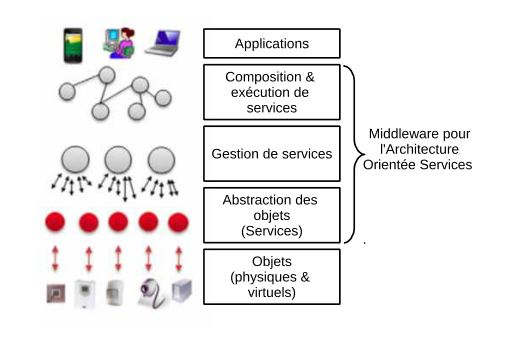
\includegraphics[width=1\linewidth]{images/MiddlewareSOA.jpg}
\end{center}
\caption{Middleware pour l’Architecture Orientée Services}
\label{fig:1}
\end{figure}

La figure 1 illustre l'architecture orientée services, la contribution de ce mémoire se positionne dans la couche Composition et exécution de services.
Cette couche fournit une composition des services et se charge du suivi de l’exécution de ces services composites. Un aspect important de cette couche est la résilience aux
pannes et l’adaptation en fonction des changements dans le système \cite{1}.



D'après l'architecture vu précédemment, Un service Web composite peut être définis comme un  résultat d’une composition de plusieurs Web services, et qui peut à son tour entrer dans une autre composition.
Les  services web composites ont pour objectif  la production des services complexes pour répondre à des demandes d’utilisateurs complexes. 

La structure d’un Web service composite peut être générée manuellement ou automatiquement. Selon les requêtes demandées, les utilisateurs peuvent spécifier manuellement comment les fonctionnalités des Web service seront combinées ou bien  un composeur qui prend la responsabilité d’une génération automatique des Web service Composite en fonction de la demande, pour qu’ils seront finalement exécuté par un moteur d’exécution.


\begin{figure}[H]
\begin{center}
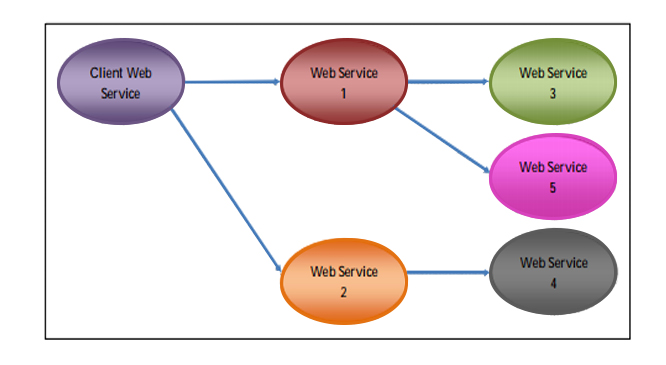
\includegraphics[width=1\linewidth]{images/CWS.jpg}
\end{center}
\caption{Web service composite}
\label{fig:2}
\end{figure}



Les Web services composite peuvent être représentés sous différents formes et structures en indiquant l’ensemble des informations et instructions relatives, comme l’ordre d’exécution et le comportement des Web services composants ainsi que les flux de données  et de contrôle.
La représentation peut être sous forme de Workflows, Graph ou réseau de Petri.



Les différents travaux et articles scientifiques sur la composition des services Web considèrent la composition de services Web comme étant un moyen efficace 
pour créer, exécuter, et maintenir des services qui dépendent d’autres services. Les auteurs ont défini le cycle de vie d’une composition de services Web reposant à partir de six activités [Benatalla] \cite{6}: 

- L’encapsulation de services natifs (Wrapping services): Cette première activité permet de  s’assurer que tout service peut être appelé lors d’ une composition, indépendamment de son  modèle de données, de son format de message, et de son protocole d’interaction. 


- L’établissement d’accord d’externalisation (Setting outsourcing agreements): Cette seconde activité consiste à négocier, établir, et appliquer des obligations contractuelles entre les services.


- L’assemblage de services composants (Assembling composite services):Cette activité permet  de spécifier, à un haut niveau d’abstraction, l’ensemble des services à composer afin d’atteindre  l’objectif attendu. Cet assemblage comporte une phase d’identification des services et de spécification de leurs interactions conformément aux descriptions et aux accords entre services. 


- L’exécution de services composants (Executing services):Cette activité consiste en l’exécution des spécifications de la composition précédemment définies. 


- Le contrôle de l’exécution de services composites (Monitoring services): La phase de contrôle permet de superviser l’exécution de la composition en vérifiant, par exemple, l’accès aux services, les changements de statut, les échanges de messages. Ce contrôle permet de détecter des violations de contrats, de mesurer les performances des services appelés et de prédire des exceptions. 


- L’évolutivité des services (Evolving services):Cette dernière phase permet de faire évoluer la composition en modifiant les altérations de l’organisation de services, en utilisant de nouveaux  services, ou en prenant en compte les retours de la phase de contrôle. \cite{6}



Dans ce mémoire, nous considérons les services avec leurs définition général c'est à dire des opérations exposées
sur Internet qui sont indépendantes de leur mise en œuvre. les détails d’implémentations telles que SOAP ou REST sont hors du domaine d’investigation de ce mémoire.

Les services sont décrits en fonction de leur fonctionnalités et des critères de qualité de service (QoS). Dans notre cas, la fonctionnalité d’un service est donnée par les paramètres d’entrée et de sortie.

\subsection { Qualité de Service }

La qualité de service (QoS Quality of Service) décrivent les caractéristiques non fonctionnelles du service Web, autrement dits la mesures dans laquelle un ensemble de caractéristiques répond à un besoin ou une attente.

nous considérons les trois critères de qualité suivantes \cite{2} :

- Temps de réponse: le temps estimé nécessaire pour achever une invocation de service ; qui est, la durée entre une demande de service et la réponse du service correspondant.

- Disponibilité : la probabilité d’obtenir une réponse correcte après une invocation de service. Cela inclut la probabilité que le service est disponible, qu’il s’exécute correctement, et que la transmission de message entre le
service et le demandeur a réussi.
 
- Prix: une mesure du coût d’exécution d’un service.


\section{Exécution tolérante aux pannes}

La tolérance aux pannes est la manière dont un système informatique, un système électronique ou un réseau répond à une défaillance matérielle ou logicielle. Le terme fait essentiellement référence à la capacité d'un système à prendre en compte les défaillances ou les dysfonctionnements d’un ou de plusieurs de ses composants, tout en fournissant un service ininterrompu, et cette capacité peut être fournie par un logiciel, un matériel ou une combinaison des deux.

Le but est d'éviter une panne catastrophique qui pourrait résulter d'un seul point de défaillance. 

\subsection{Défaillance des Web Service Composite}

Comme toutes les technologie, Les Web services Composite ne peuvent pas s’échapper aux défaillances d’exécution à 100 \%, car des pannes peuvent survenir à tout moment au niveau du matériel, du moteur d’exécution ou tout simplement du défaillance d’un Web service composant.
Cependant les Web Services Composite fonctionne potentiellement de manière réduite (en mode dégradé).


Soulever et relever les défis posés par les problématiques de résilience et de fiabilité des web services composite nécessite en premier lieu l’analyse  des caractéristiques des pannes dans  leur exécution.
On peut distinguer principalement dans l’environnement d’exécution des Web services Composites deux classe de pannes \cite{2}. 

    - Panne de nature silencieuse: (silent faults) Sont les pannes indétectables, ou qui sont détectées après une très grande durée depuis leurs déclenchements ce qui implique nécessairement que le résultat fourni est incorrect. 
    Ces pannes sont génériques pour tous les WS. Ils empêchent les WS de répondre.


    - Panne de nature logique: (Logic fault): Contrairement au pannes silencieuse, les panne logiques sont spécifiques aux différents Web service, et les attributs des entrées représente la cause principale de ces pannes.
    Ce genre d’erreur est difficile d’être identifié par le moteur d’exécution des Web services composites.

\subsection{Exécution tolérante aux pannes des CWS}

Le contrôle d'exécution des Web services composites peut être centralisé c’est à dire un coordinateur qui va jouer le rôle de la gestion de toute l’exécution,  ou distribué dans lequel le processus d’exécution de déroule avec la collaboration de plusieurs participants sans un coordinateur central. Comme il peut être attaché aux web services composants ou indépendant.
Certaines méthodes indépendantes de tolérance aux pannes dont apparus, telles que les propriétés transactionnelles et la réplication. Les propriétés transactionnelles décrivent implicitement le comportement des services web en cas d'échec, et sont utilisées pour garantir la propriété transactionnelle d’atomicité.

Les propriétés transactionnelles les plus utilisées pour les services web sont pivot, compensable, et retriable [Rafael Enrique Angarita Arocha],[modeling dinamic ...] \cite{1}. 
 
 - Pivot(p) : un service est appelé pivot si ses effets restent pour toujours
et ne peuvent pas être annulés sémantiquement une fois qu’il a terminé son exécution avec succés. Il s’agit de la propriété transactionnelle la plus basique.

- Compensable (c) : un service est compensable s’il existe un autre service qui peut sémantiquement annuler son exécution s'il n'as pas pu terminer avec succès.  
 
- Retriable (r) : un service est retriable s’il garantit une exécution réussie après un nombre fini d’invocations. Cette propriété doit être combinée avec les propriétés pivot ou compensable, créant les propriétés pivot-retriable (pr) et compensable-retriable (cr).

Les services Web composites sont construit à partir d'un ensemble des service qui offrent des propriétés transactionnelles garantissent la cohérence su système et ont une propriété transactionnelle agrégée comme suit [Rafael Enrique Angarita Arocha]: 

- Atomique : un service composite est atomique si au moins un de ses services composant est pivot ou pivot retriable. Lorsqu’un service composite atomique se termine avec succès, ses effets demeurent pour toujours et ils ne peuvent pas être annulées. Si l’un de ses services composants tombe en panne, le système est laissé dans un état sémantiquement similaire à celui qu’il avait avant l’exécution du service composite.


- Compensable : un service composite est compensable si tous ses services composants sont compensables. Cela signifie qu’il existe un autre service composite, contenant les services qui compensent les services du service composite compensable, qui peut annuler sémantiquement les effets du service composite compensable après son exécution réussie. Comme pour le service composite atomique, si l’un de ses service composants tombe en panne, le système est laissé dans un état sémantiquement similaire à celui qu’il avait avant l’exécution du service composite compensable.


- Retriable : un service composite est retriable si tous ses services composants sont retriables. Un service composite retriable garantit l’exécution réussie après un laps de temps limité. Cette propriété doit être combinée avec les propriétés atomiques ou compensables, pour créer les propriétés atomique-retriable (ar) et compensable-retriable (cr).


\section{Mécanisme de récupération}

En présence des pannes, les propriétés transactionnelles fournis par les services ont une importance dans la création des services composites fiables, car ils assurent un état cohérent de l'ensemble du système.

La stratégie de reprise d'une exécution de service composite dépend de la propriété transactionnelle des services composants.
Les principaux mécanisme de récupération sont \cite{1} : 

- Récupération en arrière : c'est l'opération de restauration de l’état du système avant l’exécution du service composite ; c’est-à-dire, tous les effets produits par le service en panne sont annulées par rollback, et les effets des services exécutés avant la panne sont sémantiquement annulés en utilisant des techniques de compensation (Fig (a)).


- Récupération en avant : c'est l'opération qui permet la réparation du panne afin que le  service composite peut poursuivre son exécution ; les techniques utilisées pour fournir une récupération en avant sont le réessayage de l’invocation de service ou le remplacement du service (Fig (b)).


- Récupération sémantique : elle a le même mécanisme que la récupération en arrière, sauf que la récupération sémantique est effectuée après une exécution réussie d’un service composite en compensant l’exécution de ses services composants. L’idée est de laisser le système dans un état sémantiquement proche de l’état qu’il avait avant l’exécution du service composite (Fig (c))

- Checkpointing : c'est l'opération qui permet si une panne survient de continuer l’exécution de la partie du service composite qui n’a pas été affecté par cette panne, tout en retardant l’exécution de la partie affectée (Fig (d))

\begin{figure}[H]
\begin{center}
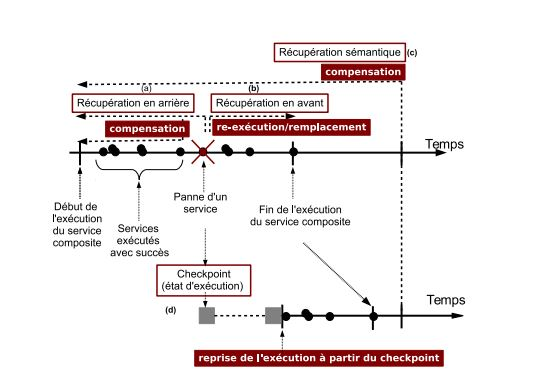
\includegraphics[width=1\linewidth]{images/techsreparation.jpg}
\end{center}
\caption{Stratégies de récupération \cite{1}}
\label{fig:3}
\end{figure}

\vspace{1cm}

\chapter{État de l'art}

\section{Introduction}

Ce chapitre présente l'étude existante avec son ensemble d'approches pour une exécution fiable des services Web composites.
Cet étude consiste l'exécution auto-corrective (self-healing) d'une manière dynamique et automatique, elle vise le même objectif de ce mémoire mais les méthodologies changent. 

Dans cette étude les chercheurs ont proposé l'approche de l'auto-corrective  (self-healing) qui se base sur les propriétés transactionnelles comme un concept de base pour une tolérance aux pannes automatique, et se base aussi sur les agents à base de connaissances.

Dans un premier temps les auteurs ont proposé une approche pour l'exécution tolérante aux pannes des services Web composite basée sur la récupération en avant et en arrière, et définie par le formalisme de réseaux de Petri Colorés, ensuite sur le même formalisme la deuxième approche consiste la proposition d'un mécanisme de point de contrôle, et finalement après une étude sur l'impact des différentes stratégies de récupération sur les services Web composite, la troisième approche apporte un modèle de décision dynamique de la stratégie de récupération en terme d'impact sur la qualité de service pour la tolérance aux pannes de services Web composites.


\section{Contrôle d'exécution de services Web composites}

En utilisant les réseaux de Petri Colorés les auteurs ont formalisé les services Web composites, leur exécution, et leurs stratégies de tolérance aux pannes, et il ont proposé un framework pour une exécution distribuée fiable et tolérante aux pannes pour les services Web Composites.

Le framework est composé de deux types de composants \cite{1} \cite{5}: 

- Un Coordinateur d'Agents : Composant responsable de la gestion des aspects globaux d'exécution des services Web composites.

- Agents de Service : ils exécutent les services et sont en charge du contrôle de l'exécution et de la tolérance au pannes.

Cette approche fournis les mécanismes de récupération en arrière par compensation, en avant par re-exécution de service et remplacement, la réplication, et le checkpointing, et assure une exécution tolérante aux pannes basé sur un modèle d'exécution distribué.

L'exécution des services Web composite peut être \cite{3} : 

- Séquentiel : Les services se basent sur les résultat des services précédents, et ne peuvent être invoqués tant que les services précédent ne sont pas terminés.

- Parallèle : Les services peuvent être invoqués d'une manière simultanée, car il n'y a pas des dépendances de flux de données entre eux.

Ces deux scénarios d'exécution ont un effet sur la propriété transactionnelle globale du service Web composite, pour cela il faut suivre le flux d'exécution défini par le graphe du service composite pour s'assurer que l'exécution séquentielle et parallèle satisfont la propriété transactionnelle globale.

\subsection{Architecture du Framework}

Les chercheurs ont proposé un Framework dont l'exécution du service composite est gérée par un Coordinateur d'Agents et une collection d'Agents de services, organisés dans architecture trois tiers.

\begin{figure}[H]
\begin{center}
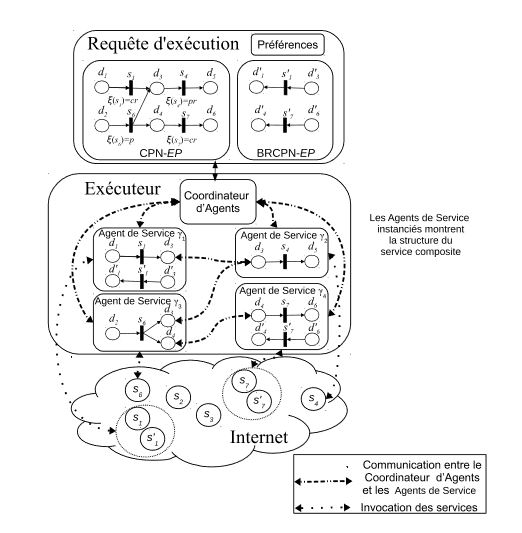
\includegraphics[width=1\linewidth]{images/architectureFrmwork.jpg}
\end{center}
\caption{Architecture d'exécution \cite{1}}
\label{fig:4}
\end{figure}


L’architecture du Framework est composée de trois niveaux principaux:

Le premier niveau : Le coordinateur d’agents reçoit le service composite et son graphe de compensation correspondant, qui sont représentés sous forme des réseau de Pétri Colorés, qui peuvent être générés d'une manière automatique ou manuelle.
Dans ce niveau le Coordinateur reçoit aussi une propriété qui lui indique si le mécanisme de checkpointing est activé ou non.

Le deuxième niveau: Le coordinateur d'Agents lance un Agent de Service pour chaque service composant du service Web composite, chaque agent de service sera responsable du contrôle de l'exécution de son service, ses rôles sont les suivants \cite{1}:

    - Responsabilité de l'invocation de services ;

    - Surveillance de l'exécution des services correspondants ;
    
    - Envoi des résultat selon le flux d'exécution ;
    
    - Lancement des stratégies de tolérance aux pannes en cas de panne.

Le troisième niveau : consiste l'interaction des agents de services avec l'ensemble des services correspondants.

L'objectif de cet architecture est de répartir la responsabilité de l'exécution d'un service Web composite à travers de plusieurs agents de service, pour que le modèle logique de l'exécuteur proposé permet une exécution distribuée et une indépendance de la mise en oeuvre 

\section{Modélisation des stratégies de récupération basées sur QoS}

Après les évolutions des recherches, les auteurs ont découvert a travers leur étude qu'il y a des impacts des différentes stratégies de récupération sur les services Web composite et plus précisément sur sa qualité de service (QoS). C'est pour cela ils ont décidé de proposer une approche pour une décision dynamique des stratégies de récupération.

Pour fournir un choix dynamique de la stratégie de tolérance aux pannes, les auteurs ont proposé une approche auto-corrective (Self-Healing) pour les services Web composites.
Dans l'auto-correctif les agents de services sont des agents basés sur des connaissances, c'est à dire ils sont basés sur l'ensemble des information qu'ils ont sur le service Web composite, sur eux mêmes, et sur ce qui est attendu et ce qu'il se passe réellement pendant l'exécution, pour qu'ils puissent finalement faire la sélection de la stratégie de tolérance aux pannes.

Indépendamment de la technique utilisée pour l'estimation des critères de Qualité de service,ils ont proposé que chaque service Web est annoté avec son temps d'exécution estimé, son prix, sa réputation et sa propriété transactionnelle. Grâce aux critères des services composants, il est possible de calculer la Qualité de service d'un service Web composite en calculant des différents critères.

Sur cette base, la conception sera sous forme d'une boucle d'auto-guérison/auto-correction par agent de service pour effectuer la détection, le diagnostic et la récupération d'une manière décentralisée \cite{1}.


\begin{figure}[H]
\begin{center}
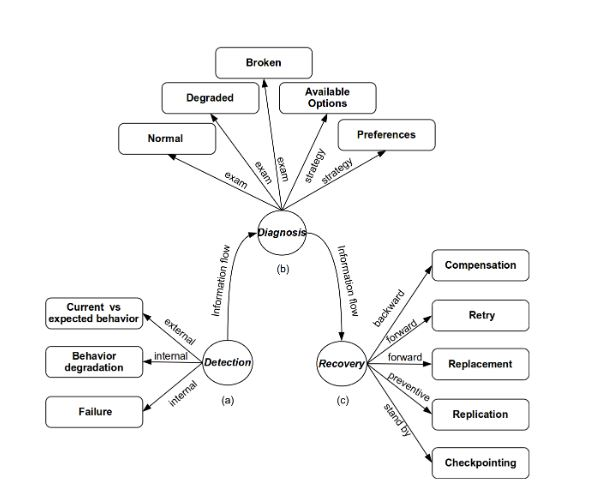
\includegraphics[width=1\linewidth]{images/Boucleauto-correctivedesAgentsdeService.jpg}
\end{center}
\caption{Architecture d'exécution \cite{1}}
\label{fig:5}
\end{figure}

- Le composant detection : Dans ce composant, trois sources sont prises en compte une externe et deux internes. 
La source externe consiste l'information sur la Qualité de service attendu, par exemple, le cas où l'utilisateur peut permettre une certaine dégradation de la Qos.
La source interne concerne la dégradation de la Qualité de service des services composants (par exemple, les variations négatives dans le temps d'exécution et le prix), et concerne aussi les pannes de services.

- Le composant diagnosis : ce composant a le rôle d'analyse du problème et la détermination de l'état du service.
Il existe trois diagnostics possibles qui correspondent au trois états d'un système auto-correctif : normal ; degraded ; et broken. Le choix de la stratégie de récupération est influencé par les options disponibles ( par exemple, les propriétés transactionnelles, les services de remplacement disponible, etc.), et influencé aussi par les préférences de l'utilisateur (la QoS attendu, le checkpointing, etc).

- Le composant recovery :  Ce composant prend en charge l'exécution des mécanismes de tolérance aux pannes sélectionnés : la récupération vers l'arrière avec la compensation ; la récupération en avant par la reexécution ou remplacement ; la prévention grâce à la réplication ; ou le retardement d'exécution par le checkpointing.



\section{Évaluation expérimentale }

Les chercheurs ont mis leur approche en évaluation expérimentale, et ça par la mise en oeuvre du Framework  en utilisant un cas d'étude qui consiste un scénario et un environnement.
L'observation du cas d'étude a été sur trois systèmes différent :

Système sans tolérance au pannes : c'est un système qui n'a aucun mécanisme de tolérance aux pannes. et dans le cas ou un des services composants tombe en panne, une exception sera générée et l'exécution sera terminé.

Système transactionnel : c'est un système qui se base sur les propriétés transactionnelles des services composants pour prendre les décisions de récupération.

Système auto-correctif :  c'est un système qui se base sur l'ensemble d'information et règle contenu dans les bases de connaissances des agents de services.


Les résultat de l'évaluation expérimentale ont montré : l'importance et la nécessité d'avoir des mécanisme de tolérance aux pannes pour les services Web composite, ainsi que la manière avec laquelle les deux approches des propriétés transactionnelles et l'auto-corrective gèrent les pannes et prennent la décision de récupération.
L'évaluation expérimentale faite pendant cette étude suggère que la combinaison des propriétés transactionnelles avec des capacités d'auto-corrective permet de donner une intelligence aux systèmes d'exécution pour gérer les exigences de haut niveau pour les exécutions de services Web composites avec une intervention humaine minimale\cite{1}.

\section{Conclusion}

Pendant cette étude, les auteurs ont proposé une approche auto corrective pour l'exécution de services Web composite qui se base sur les propriété transactionnelles des services Web composants ainsi que sur une base d'informations sur les Services Web qui se présente principalement dans la Qualité de chaque service QoS.

L'avantage principale de cette étude c'est la mise en oeuvre des mécanismes de d'exécution et de récupération qui sont capables de fonctionner d'une manière automatique, ces mécanismes sont mis en place a travers un Framework qui se base sur des agents de services qui sont en charge du contrôle de l'exécution  et de la tolérance en pannes, ces agents prennent un ensemble d'informations en entrée pour qu'il puissent les analyser et en déduire des nouvelles informations qui vont permettre une prise de décision lors de l'exécution.

Cet étude est considérée comme une base pour le sujet de recherche du présent mémoire, qui visent le même objectif de l'auto-corrective, et qui se situe dans les principaux perspectives de cette étude.

Le mémoire est l'un des principaux perspectives de l'étude présentée dans l'état de l'art car il se base sur l'ensemble des données générées par le système d'exécution de services Web composites mis en place pendant l'étude expérimentale précédente. Donc l'objectif sera collecter et stocker les données générées, les traiter et les analyser à l'aide des outils de l'auto apprentissage (Machine Learning) pour en pouvoir prédire la bonne décision de stratégie de récupération.





\chapter{La prédiction du mécanisme de récupération}

\section{Introduction}
Notre étude a pour objectif la prédiction de la meilleure stratégie de récupération en cas de pannes dans un Web Service Composite en se basant sur un ensemble d'informations concernant les services Web composants et leurs qualités de services.

L'approche proposée par le présent mémoire se base sur les notions de l'auto-apprentissage (Machine Learning). L'ensemble des données générées dans l'étude précédente ( cité dans le chapitre "État de l'art"), seront traitées et exploitées pour un apprentissage, afin de prédire d'une manière automatique et dynamique le mécanisme de récupération le mieux adapté.

ce chapitre présente les différents types de problèmes d'auto-apprentissage, et la famille de problématique dans laquelle s'oriente notre approche de prédiction,et décris les deux étapes principales de l'approche, le traitement et l'intégration des données en utilisant Pentaho et la prédiction des mécanismes de récupération en appliquant les algorithmes de Machine Learning via l'outil Weka. 


\section{L'auto Apprentissage -Machine Learning- }

L'apprentissage automatique -Machine Learning- est un domaine de l'intelligence artificielle qui consiste en général une manière de traitement d'un ensemble de données pour un apprentissage automatisé de la machine ou de l'ordinateur afin de pouvoir effectuer des opérations complexes.

Un algorithme de machine Learning se différencie des autres algorithmes classiques à travers la notion de l'apprentissage, car un algorithme de Machine Learning s'améliore par lui même à partir des données sans supervision d'un être humain.

Pour bien définir un problème de machine learning, il faut bien définir quatre éléments principaux: 

- Les données

- La tache à accomplir 

- L'algorithme d'apprentissage

- La mesure de performance


Les données : représente l'ensemble de base d'information sur lesquelles se base l'apprentissage automatique, notre approche se base sur les données générées par le système d'exécution des services Web Composite cité dans l'Etat de l'art.

La tache spécifique : Le Machine Learning a besoin de la définition d'une tâche spécifique à accomplir c'est à dire  qu'est ce qui peut répondre au problème, une tâche peut être sous forme d'une prédiction, identification, recommandation... 

L'algorithme : Après la définition de la tâche spécifique et les données nécessaires pour la traiter, On peut passer à la troisième étape qui consiste le choix d'un algorithme spécifique qui va pouvoir répondre à la tache à partir des données collectée. il existe plusieurs algorithmes de Machine Learning ( Réseau de neurones, Support vector machine, Régression linéaire ... ), le choix de l'algorithme dépend de la nature et le type de la problématique de machine Learning.

La mesure de performance : Une fois l'algorithme est déterminé, il faut choisir une mesure de performance relativement à la tache définie précédemment en s'appuyant sur des métriques précises.  

Un process de Machine Learning passe par deux phases principales, La première phase c'est la phase où l'être humain sera responsable du choix et de l'entraînement de l'algorithme d'apprentissage, pour que le traitement de la tache spécifique sera appris à partir de l'apprentissage (Training set), pour que l'algorithme dans la deuxième phase effectue la tâche lui même.

\begin{figure}[H]
\begin{center}
\includegraphics[width=1\linewidth]{images/auto apprentissage.png}
\end{center}
\caption{Processus du Machine Learning}
\label{fig:6}
\end{figure}


\subsection{Base d'information de contexte des Services Web Composite}

La prédiction de la stratégie de récupération va être basée sur un ensemble de données de base de connaissances des services Web composites.

D'après l'approche de l'auto-corrective (self-healing) citée dans le chapitre précèdent, qui démontre et étudie l'impact des stratégies de récupération sur les services composites, et propose un modèle de décision de mécanisme de récupération en terme d'impact sur la QoS des services composites, dans cette approche, les agents de service sont agents qui se base dur des connaissance. ils décident la stratégie de tolérance aux pannes en se basant sur les information qu'ils ont sur eux-même, sur le service Web composite, et sur ce qui est attendu et ce qu'il se passe réellement pendant l'exécution.\cite{1}

Notre Approche va se baser sur l'ensemble des données générées précédemment par ce système d'exécution, qui décrivent le comportement des services Web composites et leurs composants, ainsi que les stratégies de récupération et leur impact sur l'exécution du service composite, pour qu'on puisse s'en servir pour l'auto apprentissage afin de prédire la récupération pour des nouvelles informations des nouveaux Web service Composite.

\subsubsection{La classification des informations de contexte}


\textbf{La qualité de service QoS :}  QoS est un ensemble des valeurs qui décrivent les caractéristiques non fonctionnelles des services Web. Nous considérons le temps d'exécution, le coût, la réputation et les propriétés transactionnelles comme des critères de QoS. Ils ont été calculés avant l'exécution des CWS, et leurs valeurs sont connues au moment de l'exécution \cite{2}

\textbf{État d'exécution :}  L'état d'exécution d'un Service Web Composite est défini en fonction de ce qui s'est passé et de ce qu'il reste à faire à un moment donné.
Prenant l'exemple du temps écoulé depuis le début de l'exécution; combien de temps estimé reste jusqu'à la fin; combien de service Web ont été exécutés; et combien de sorties utilisateur ont été générées. Ces paramètres sont calculés lors de l'exécution d'un CWS en tant que valeurs agrégées tandis que les WSs de composants sont exécutés avec succès.

\textbf{État d'environnement :} Consiste l'ensemble des conditions que le système possède lors d'une exécution d'un service Web Composite. Ces conditions sont indépendantes des services Web composites et des valeurs QoS attendues de ses composants.


Chaque service Web a sa propre estimation d'exécution (temps, coût, réputation, propriété transactionnelle. 

\begin{itemize}
\item [$\bullet$] Temps d'exécution estimé : \textit{WSetime}

\item [$\bullet$] Coût  :\textit{WScost}

\item [$\bullet$] Réputation : \textit{WSrep} est une agrégation des feedbacks des utilisateurs, elle reflète la fiabilité et la crédibilité du service et de son fournisseur.

\item [$\bullet$] Propriété transactionnelle : \textit{TP(WS)} c'est la propriété transactionnelle qui décrit le comportement du service Web dans le cas de pane. Il peux être pivot (p), compensable (c), pivot retriable (pr), ou compensable retriable(cr). 

\end{itemize}

Après la détermination des critères de QoS de chaque service Web, il est possible maintenant de calculer la QoS globale pour le service Web composite, en calculant le temps total d'exécution CWSETime, le coût total CWSTcost et la réputation total CWSTrep.

\begin{itemize}
\item [$\bullet$] Qualité associée à un service Web composite : \textit{Q} 

$$
 Quality(cwsQ) = w1 \ast CWSETime + w2 \ast CWSTCost + w3 \ast CWSTREP   \cite{2}
$$
 
 La qualité associée à un service Web Composite dépend des critères de qualité de service et de la pondération de ces critères. w1, w2 et w3 sont les poids pour le temps d'exécution, le prix et la réputation.
 
\item [$\bullet$] QoS degré de tolérance aux pannes pour un CWS \textit{ $$ \Delta QoS(cws) $$ }  Représente la valeur agrégée maximale de QoS autorisée à dépasser pour l'exécution d'un CWS. Il est exprimé en pourcentage de qualité.

\item [$\bullet$] QoS supplémentaire tolérée d'un CWS  \textit{CWSExtraQoS}  : Soit cws un le service Web composite, Quality (cwsQ) sa QoS agrégée, et son degré de QoS maximum supporté, CWSExtraQoS est définis comme suit: 

  $$ CWSExtraQoS(cws) = QualityQ(cws) + \Delta QoS(cws) $$
 
\item [$\bullet$] Temps réel exécuté d'un CWS \textit{WSRET} : WSiRET fait référence au temps réel investi depuis que wsi a été invoqué jusqu'à ce qu'il finisse. S'il se termine avec succès,c'est le temps entre le moment où il a reçu toutes ses entrées jusqu'à ce qu'il envoie ses sorties produites. En cas d'échec, c'est le délai entre le moment où il a reçu toutes ses entrées jusqu'à ce qu'une panne soit détectée.


\item [$\bullet$]Temps d'exécution réel passé d'un WS  \textit{WSPT} : Soit WSi un composant WS dans un CWS; WSiPT fait référence au temps réel investi depuis que le CWS commence son exécution, de Ni, jusqu'à ce que WSi soit invoqué.

\item [$\bullet$] Temps restant estimé d'un WS  \textit{WSRemainT} : Soit WSi un composant WS dans un CWS; WSiRemainT est la valeur maximale entre tous les chemins séquentiels de WSi à Nf.

WSiRemainT permet de regarder en avant et de calculer à quel point en termes de temps d'exécution est la fin d'une exécution CWS par rapport à chaque composant WS.

\item [$\bullet$]Temps Degré de tolérance aux pannes d'un WS \textit{$$\Delta Time (wsi)$$} Soit cws un Service Web Composite avec CWSExtraQoS (cws). Soit wsi un composant WS de cws avec: WSiPT; WSiRemainT; WSiRET; et WSiETime. Temps Degré de tolérance aux pannes  représente le temps maximum autorisé pour dépasser l'exécution de wsi pour satisfaire CWSExtraQoS (cws); il est exprimé comme:


$$ \Delta Time(wsi) = CWSExtraQoSTime(cws) - w1 $$  $$ \ast(WSiPT + WSiRemainT + WSiRET +  WSiETime) $$



\item [$\bullet$] Connectivité réseau actuelle à un WS  \textit{WScomm} : Soit I (wsi) et O (wsi) les entrées et les sorties d'un WS wsi; la connectivité réseau actuelle de wsi (WSicomm) est le temps de transfert estimé de I (wsi) et O (wsi) entre le "moteur d'exécution" et wsi.

\item [$\bullet$] Degré de dépendance en sortie d'un WS  \textit{WSOD} : WSiOD est le nombre de sorties CWS qui dépendent d'une exécution réussie de wsi. Ce degré reflète l'importance d'un WS en termes de nombre de sorties utilisateur qui dépend de son exécution réussie.

\end{itemize}


Les variables citées ci-dessus représentent les variables les plus pertinentes sur lesquelles on peux se baser pour prendre une décision de choix de stratégie de récupération.

\subsection{Traitement et intégration des données }

Les données collectées pour notre approche de décision, sont des données générées par le système d'exécution proposé dans l'approche d'auto guérison, les données obtenues ne sont pas forcement des données structurées et pertinentes pour notre objectif. 

Le but de cette phase de traitement est la structuration des données et l'extraction des variables pertinentes pour notre prise de décision pour en pouvoir construire notre propre entrepôt de données, pour cela on utilisera l'outil Pentaho Data Integration. 

\subsubsection{Pentaho Data Integration }

Pentaho Data Integration est un ETL open source d'intégration de données qui permet d'extraire les données depuis différents sources, en exécutant des opérations de manipulation et de transformation de données, pour les adapter et les charger dans un entrepôt de données.

Pentaho fonctionne sur un modèle graphique a base d'étape, il donne la possibilité de création de processus de transformation, d'importation ou d'exportation des données sans programmation.

L'outil Pentaho Data Integration offre des fonctionnalités de préparation des données : 

\begin{itemize}
    \item L'extraction
    \item La transformation 
    \item Le chargement des données 
\end{itemize}

Et permet la création de deux types de processus : 

\begin{itemize}
    \item Les transformations : c'est l'ensemble des opérations effectuées sur un les données, qui comprennent le chargement et la lecture des données, la manipulation et l'écriture de ces dernières.
    
    \item Les taches :  est un traitements qui combine des actions telles que l'exécution d'une transformation Pentaho Data Integration, l'envoi d'un mail, le téléchargement d'un fichier ou le lancement d'une application.
    
\end{itemize}

\textbf{Utilité :}

Pour notre mémoire, l'utilité de Pentaho c'est le pouvoir de collecter et intégrer l'ensemble des données concernant les Services Web Composites, et leurs services composants. Ensuite l'extraction des variables pertinentes citées au dessus, pour qu'on puisse avoir un entrepôt de données final, qui va s'en servir comme un échantillon d'apprentissage.


\subsection{Choix de l'algorithme de Machine Learning}

Le choix de l'algorithme auquel  on va avoir besoin de faire appel pour le traitement de la problématique nécessite tout d'abord  la distinction des différents types de problèmes de Machine Learning et les familles d'algorithmes associés avec leurs spécificités.

La première distinction à faire dans les problèmes de Machine Learning, c'est la détermination des problèmes supervisés (supervised learning) et des problèmes non supervisés (unsupervised learning), la seconde consiste la distinction entre un problème de Régression et un problème de Classification \cite{ML}.

\subsubsection{Apprentissage supervisé vs non-supervisé}


- \textbf{L'apprentissage supervisé : }exploite exclusivement l'ensemble des données dites annotées de leur sorties pour pouvoir construire un modèle, c'est à dire que chaque donnée est associée à une classe cible ou une catégorie et l'objectif c'est que l'algorithme soit capable de prédire cette classe sur des nouvelles données qui ne sont pas annotées a partir du modèle qui a construit précédemment.

\textit{Représentation Mathématique :} 
    
    On reçoit en entré des données d'exemple annotées:
    (x1,y1),(x2,y2),(x3,y3), ... et on veut prédire la sortie sur des nouvelles données :  x* --> y* 
    

- \textbf{L'apprentissage non-supervisé : } est beaucoup plus complexe puisque les données d'entrées ne sont pas annotées. l'algorithme d'entraînement va devoir dans ce cas  trouver  les similarités et distinctions au sein de ces données, et à organiser et regrouper ensemble celles qui partagent des caractéristiques communes.

\textit{Représentation Mathématique : }
    
    On reçoit en entré uniquement des données brutes de variables aléatoire : x1,x2,x3,... et on veut avoir la relation avec des variables latentes structurelles :  xi --> yi 
    
En plus de ces deux principales familles d'algorithmes (Supervisé/non-Supervisé) il existe d'autre types d'apprentissage, l'apprentissage semi-supervisé qui prend en entré un mélange de données annotées et non annotées, et l'apprentissage par renforcement qui se base sur un cycle d'expériences et de récompenses, et s'auto améliore à chaque itération.

\subsubsection{Classification vs Régression }

\begin{figure}[H]
\begin{center}
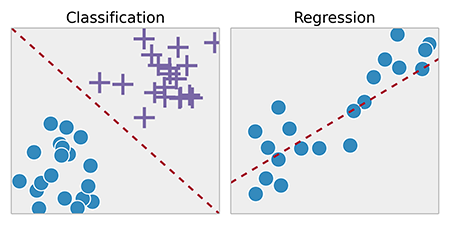
\includegraphics[width=0.8\linewidth]{images/ClassReg.png}
\end{center}
\caption{Différence entre Classification et Régression}
\label{fig:6}
\end{figure}

- \textbf{Classification :} Chaque observation ou donnée  est associée à une et une seule modalité (appelée classe/catégorie), La classification c'est le type de problème dans lequel la sortie attendu de l'algorithme est discrète c'est à dire elle est sous forme d'une catégorie ou classe.
    
    
- \textbf{Régression :} La variable de sortie de l'algorithme est quantitatif, c'est à dire elle  prend des valeurs dans un sous-domaine de l’ensemble des nombres réels. exemple: La prédiction de la rentabilité d'une compagne marketing. 


Notre problématique est la prédiction de la stratégie de récupération d'un service Web composite, c'est à dire prédire le mécanisme de récupération qui va être mis en oeuvre en cas de panne, nos données d'apprentissage sont des données générées par  un exécuteur des services Web composites vu dans l'étude précédente (Chapitre :État de l'art), qui permet de prendre la décision de choix de mécanisme de récupération, ce qui va nous permettre d'avoir un ensemble des données annotées par leur catégories de récupération. 

D'après cet analyse on peut situer notre problème de Machine Learning dans la famille des problèmes Supervisés de Classification.

\subsubsection{Les algorithmes Supervisé de Classification}

Il existe plusieurs algorithmes qui permettent la construction d'un modèle de classification, on  a sélectionne les six algorithmes les plus importants pour notre problématique de classification : 

   	
\textbf{Forêt aléatoire (Randomforest) :}

L’algorithme des forêts aléatoires ou forêt d’arbres décisionnels (Random Forest ) est un algorithme très récent (2000) pour la  classification et la régression, Random Forest utilise des stratégies de bagging c'est à dire c’est de faire la moyenne des prévisions de plusieurs modèles indépendants pour réduire la variance des prévisions d'un arbre de décision et donc l’erreur de prévision, améliorant ainsi leurs performances.

Cet algorithme est particulièrement performant pour les problématiques de prédiction, il effectue un apprentissage en parallèle sur plusieurs arbres de décision construits d'une façon aléatoire et entraînés sur des sous-ensemble de données différents, ensuite Les prédictions sont moyennées lorsque les données sont quantitatives ou utilisés pour un vote pour des données qualitatives, dans le cas des arbres de classification. L’algorithme des forêts aléatoires est connu pour être un des classifieurs les plus efficaces\cite{RF}.


\begin{figure}[H]
\begin{center}
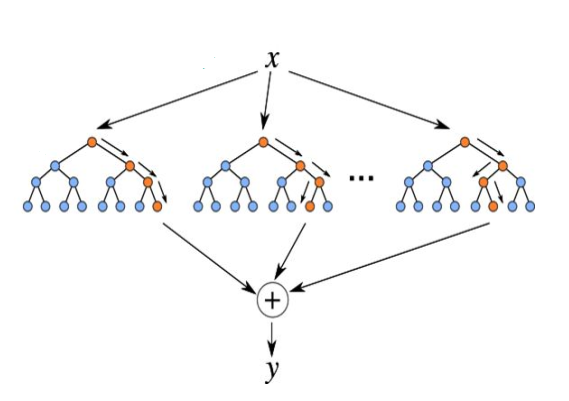
\includegraphics[width=0.8\linewidth]{images/randomforest.png}
\end{center}
\caption{Algorithme des Forêts aléatoires}
\label{fig:7}
\end{figure}

\textbf{L'arbre de décision (Decision tree) : }

Les arbres de décision sont un type d'apprentissage automatique supervisé où les données sont divisées en continu selon un certain paramètre. L'arbre peut être expliqué par deux entités, à savoir les nœuds de décision et les feuilles. Les feuilles sont les décisions ou les résultats finaux. Et les nœuds de décision sont la partie ou les données sont divisées.

\begin{figure}[H]
\begin{center}
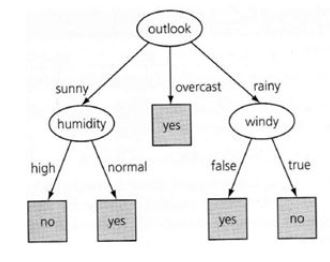
\includegraphics[width=0.8\linewidth]{images/treedecision.JPG}
\end{center}
\caption{Algorithme des arbres de décision}
\label{fig:8}
\end{figure}


\textbf{Machine à vecteurs de support (Support vector machines ) : }

Support Vector Machine (SVM) est un algorithme d'apprentissage automatique supervisé qui peut être utilisé pour les défis de classification ou de régression. Cependant, il est principalement utilisé dans les problèmes de classification. Dans cet algorithme, chaque élément de données est tracé comme un point dans un espace à n dimensions (où n est le nombre d'entités) avec la valeur de chaque entité étant la valeur d'une coordonnée particulière. Ensuite, une classification est effectuée en trouvant l'hyper-plan qui différencie très bien les deux classes

Les vecteurs de support sont les coordonnées de l'observation individuelle. Support Vector Machine est une frontière qui sépare le mieux les deux classes (hyper-plane / ligne).


\begin{figure}[H]
\begin{center}
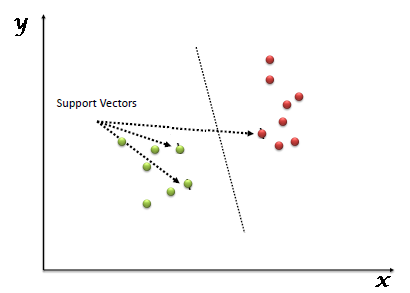
\includegraphics[width=1\linewidth]{images/SVM.png}
\end{center}
\caption{Algorithme de Machine à vecteurs de support}
\label{fig:9}
\end{figure}



\textbf{Réseau de neurones (neural network) : }

Il y a eu récemment un grand Buzz autour des "réseaux de neurones" dans le domaine de l'informatique et plus précisément dans domaine du Machine Learning, et il a attiré beaucoup d'attention de la part de nombreuses personnes.

Essentiellement, les réseaux de neurones sont composés de couches d'unités de calcul appelées neurones, avec des connexions dans les différentes couches. Ces réseaux transforment les données jusqu'à ce qu'ils puissent les classer comme une sortie. Chaque neurone multiplie une valeur initiale par un certain poids, somme les résultats avec d'autres valeurs arrivant dans le même neurone, ajuste le nombre résultant par le biais du neurone, puis normalise la sortie avec une fonction d'activation.

\begin{figure}[H]
\begin{center}
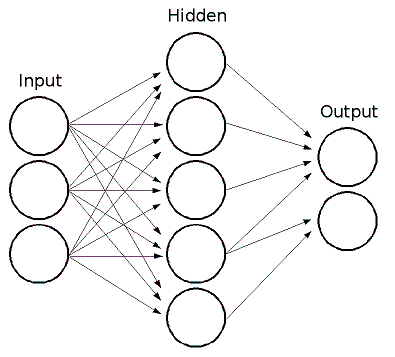
\includegraphics[width=0.7\linewidth]{images/RN.png}
\end{center}
\caption{Algorithme de Réseau de neurones}
\label{fig:10}
\end{figure}


Les réseaux de neurones se caractérise par un processus d'apprentissage itératif dans lequel les enregistrements (lignes) sont présentés au réseau une seule fois, et les poids associés aux valeurs d'entrée sont ajustés à chaque fois. Après que tous les cas sont présentés, le processus est souvent répété. Pendant cette phase d'apprentissage, le réseau s'entraîne en ajustant les poids pour prédire l'étiquette de classe correcte des échantillons d'entrée.

Les avantages des réseaux de neurones comprennent leur grande tolérance aux données bruitées, ainsi que leur capacité à classer les modèles sur lesquels ils n'ont pas été formés.


\textbf{Les K plus proches voisins (K-Nearest Neighbors KNN) :}

K plus proches voisins est un algorithme d’apprentissage supervisé. En abrégé k-NN ou KNN.
Le fonctionnement de cet algorithme se base sur un ensemble de données d'apprentissage constituée de N couples «entrée-sortie». Pour estimer la sortie associée à une nouvelle entrée x, l'algorithme des k plus proches voisins se base sur la mesure de similarité, et prend en compte (de façon identique) les k échantillons d'apprentissage dont l’entrée est la plus proche de la nouvelle entrée x, selon une distance à définir.


\begin{figure}[H]
\begin{center}
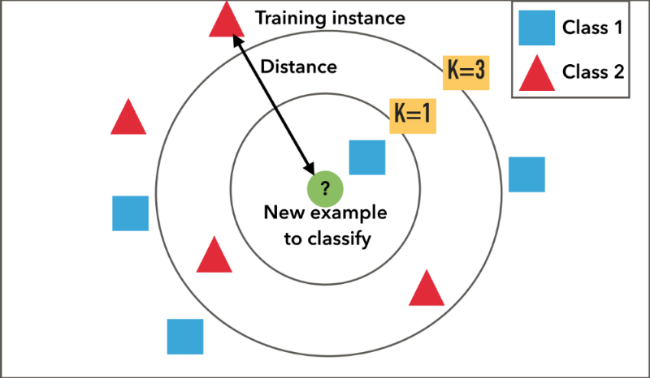
\includegraphics[width=1\linewidth]{images/KNN.png}
\end{center}
\caption{Classification par KNN}
\label{fig:10}
\end{figure}


Par exemple, dans un problème de classification, on retiendra la classe la plus représentée parmi les k sorties associées aux k entrées les plus proches de la nouvelle entrée x.

\textbf{Classification naïve bayésienne (Naive Bayes Classification) : }
    
L'algorithme de naïve Bayes est un algorithme de classification supervisée qui se base sur le théorème de Bayes. Ce dernier est considéré comme un résultat de base en théorie des probabilités. Ce théorème est fondé sur les probabilités conditionnelles qui consiste à savoir la probabilité qu'un événement se produise sachant qu'un autre événement s’est déjà produit.


La classification Multiple de Naive Bayes,  calcule le résultat en se basant sur plusieurs variables. L’application du théorème de Bayes sur plusieurs variables rend le calcul complexe. Pour contourner cela, une approche consiste à prendre en considération ces variables indépendamment les unes des autres. Il s’agit d’une hypothèse forte.

Généralement, les variables prédictives sont liées entre elles. Le terme “naïve” vient du fait qu’on suppose cette indépendance des variables.\cite{NB}


\section{Construction du modèle de prédiction}

Cette partie consiste l'exécution des algorithmes de classification cités dans la section précédente, afin de pouvoir choisir l'algorithme le plus performant pour notre échantillon de données. 

Pour l'exécution de ces algorithmes, on utilisera  Pentaho, l'outil utilisé précédemment dans l'intégration des données, qui offre une extension dédiée au data Mining. 

Après l'exécution de chaque algorithme de Machine Learning, on est censé choisir un outil de mesure de performance, pour qu'on puisse choisir un ou les algorithmes les plus performants pour notre problématique. 

\subsection{WEKA}

Pentaho Data Mining, est basé sur le projet WEKA, c'est un ensemble complet d'outils pour l'apprentissage automatique et l'exploration de données. Sa large gamme de règles de classification, de régression, d'association et de clustering peut être utilisée pour mieux comprendre l'activité et être exploitée pour améliorer les performances futures grâce à l'analyse prédictive.

WEKA est un outil qui permet d'exécuter des algorithmes de Machine Learning sur un ensemble de données. Il est ainsi possible d’isoler des populations ou d’extraire des règles à partir des données contenues dans un entrepôt de données. 

WEKA est présenté sous forme d’une application indépendante, disposant d’une interface utilisateur graphique ou en ligne de commande.


\begin{figure}[H]
\begin{center}
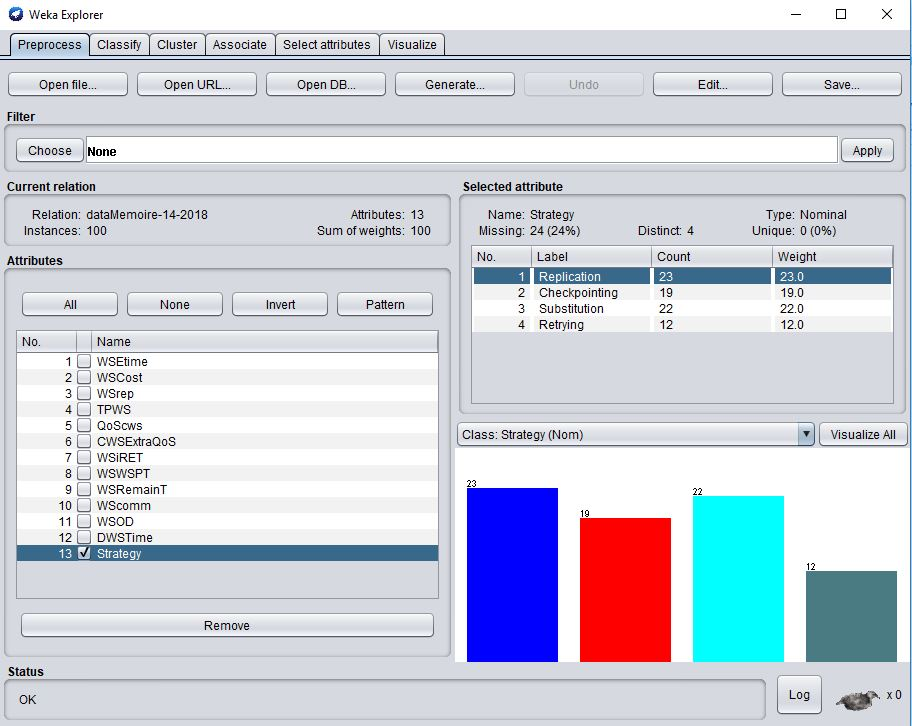
\includegraphics[width=1\linewidth]{images/weka1.JPG}
\end{center}
\caption{Importation des données sur Weka}
\label{fig:11}
\end{figure}

Après l'importation des données dans WEKA, ce dernier offre a travers les six onglets au-dessus les différentes étapes du processus d'apprentissage, soit un apprentissage supervisé ou non. 

Le premier onglet "Preprocess" permet la saisie des données, l'analyse et la sélection des attributs. 

Une fois les données sont chargées, une liste des attributs apparaît à gauche de la fenêtre, et un certain nombre de statistiques à droite qui présentent les valeurs maximales, minimales et moyennes.
En bas de la fenêtre, Weka présente un histogramme qui indique la répartition des exemples pour l'attribut sélectionné, la couleur indique la proportion d’éléments de chaque classe dans chaque colonne. On peux visualiser tous les histogrammes en même temps, cela nous donne une idée sur la répartition des données par classe (Stratégie de récupération) et par attribut. 

La figure ci-dessus, présente l'histogramme de répartition par la classe "Strategy", qui se compose de quatre catégories (Replication, Checkpointing, Substitution, Retrying), et qui sont présentées par quatre couleurs différentes. 

\subsubsection{Classification WEKA}

Le deuxième onglet de Weka "Classify" permet d'accéder à la fenêtre où on peut exécuter les algorithmes de classification sur nos données afin de construire notre modèle, c'est la partie dans laquelle on va tester tous nos algorithmes cités dans la section précédente.

\begin{figure}[H]
\begin{center}
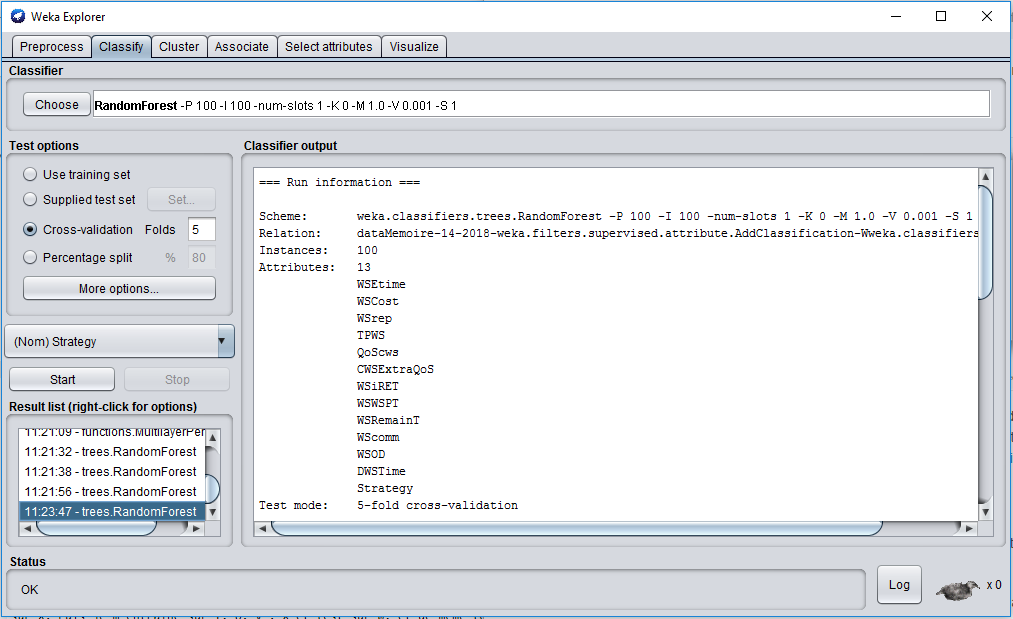
\includegraphics[width=1\linewidth]{images/wekaClassifier.PNG}
\end{center}
\caption{WEKA Classifier}
\label{fig:12}
\end{figure}

Dans cet étape on va exécuter tous les algorithmes précédents on choisissant une option de test pour les données, pour qu'on puisse faire une comparaison qui se base sur une mesure de performance qui sera à la fois la mesure de précision et la matrice de confusion. 

\textbf{Options de Test :}


\begin{figure}[H]
\begin{center}
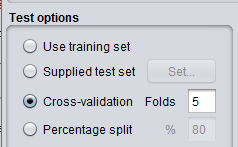
\includegraphics[width=0.5\linewidth]{images/TestOptions.PNG}
\end{center}
\caption{Options de Test WEKA}
\label{fig:13}
\end{figure}


Généralement, quand on utilise un algorithme d'apprentissage automatique, il faut en avoir des données d'apprentissage et des données de test. afin de permettre a WEKA de faire le test après la phase d'apprentissage, il faut l'informer a travers des options de la procédure à suivre concernant les données de test qui seront utilisées.

WEKA dispose de quatre options de test : 

\begin{itemize}

\item \textbf{Use training set : }  Signifie que le test sera sur les mêmes données qu'on a exploitées dans l'apprentissage. 

Généralement, cette option n'est pas performante pour une vrai évaluation d'algorithme, car on reste sur les même données.
Elle est utilisée que lorsqu'on dispose de toutes les données et qu'on souhaite créer un modèle descriptif plutôt qu'un modèle prédictif. Parce qu'il y a toutes les données, et on aura pas besoin de faire de nouvelles prédictions. Ce qui n'est pas le cas pour notre problématique de prédiction, donc cette option ne sera pas prise en compte dans notre étude.


\item \textbf{Supplied test set : }   Il s'agit d'un fichier externe qui contient des données de même modèle que les données d'apprentissage, sauf qu'elles ne sont pas annotées.

Cette Option est pratique lorsque les données sont très volumineuses, et pas un besoin de tout les exploiter pour former un modèle.

Nous disposons dans un premier temps d'un échantillon de données qui est limité et que l'on utilise pour l'apprentissage. L'option Supplied test Set n'est pas convenable avec nos conditions.


\item \textbf{Percentage split : } fractionne les données et sépare un x\% des données pour l'apprentissage et le reste pour les tests. C'est utile quand l'algorithme est lent.
Excellent à utiliser pour avoir une idée rapide de la performance d'un modèle. Il n'est pas utilisé pour prendre des décisions, du coup il se sera pas utile pour notre étude.

\item \textbf{Cross-validation : }C'est un processus qui divise l'échantillon d'apprentissage original en K échantillons, le K est nombre précisé dans "Folds".  
En prenons Folds = 5, les données seront divisées en 5 sous échantillons, et pendant 5 itérations, on prend 4 sous échantillons pour apprentissage et un seul pour le test \cite{7}.

C'est la méthode d’estimation de fiabilité de test la plus utilisée. Elle fournit généralement une estimation plus précise de la performance que les autres techniques. Ne doit pas être utilisé lorsqu'il y a une très grande quantité de données. Les valeurs communes pour k sont 5 et 10, selon la taille de l'ensemble de données. Donc la validation croisée répondra bien a notre besoin pour avoir une estimation plus précise. 

\end{itemize}

D'après le comparatif d'options fait ci-dessus, on constate que l'option la plus adaptée pour notre objectif et pour notre nature de données sera la validation croisée, en prenant un  K=5 car a priori on a pas une grande masse de données.

\subsection{Mesure de performance}


Le but de la modélisation prédictive de la stratégie de récupération des services Web composites est de créer un modèle qui fonctionne le mieux dans une situation que nous ne comprenons pas complètement, avec des nouvelles données et informations concernant les QoS des Services Web qui sont inconnues. Nous devons utiliser des techniques statistiques puissantes pour estimer au mieux la performance du modèle.

WEKA fourni un résumé des performances lorsqu'on évalue un modèle, dans l'onglet "Classifier" après avoir cliquer sur le bouton "Start", les résultats sont présentés dans le volet "Classifier Output".

Ce volet contient beaucoup d'informations, notamment:

- Les informations d'exécution telles que l'algorithme et sa configuration, l'ensemble de données et ses propriétés ainsi que l'option de test.

- Les détails du modèle construit, le cas échéant.

- Le résumé de la performance, y compris un ensemble de mesures différentes.

Lorsqu'on évalue un algorithme de Machine Learning sur un problème de classification, On reçoit une grande quantité d'informations sur les performances à assimiler.


\begin{figure}[H]
\begin{center}
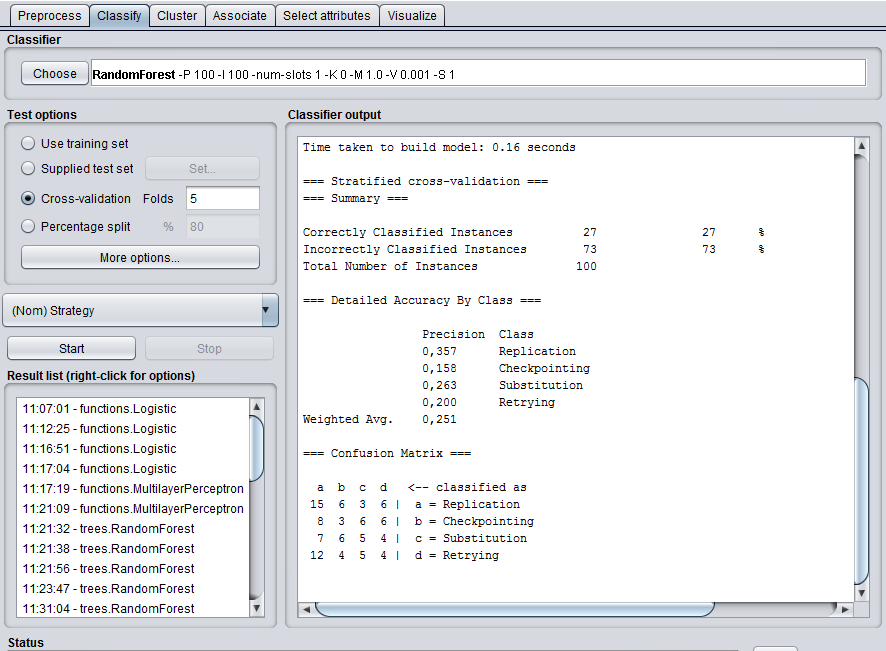
\includegraphics[width=1\linewidth]{images/summaryPerf.PNG}
\end{center}
\caption{Résumé des performances de classification pour un modèle}
\label{fig:14}
\end{figure}

Pour la classification, il existe trois aspects principaux dans le bilan de performance du modèle:

\begin{enumerate}
\item La précision de classification - Classification accuracy - : C'est le ratio entre le nombre de prédictions correctes et toutes les prédictions faites, souvent présenté sous forme d'un pourcentage où 100\% est le meilleur qu'un algorithme peut atteindre.

\item La précision par classe - Accuracy by class - : Représente le taux vrai-positif et faux-positif pour la prédictions de chaque classe, ces pourcentage peuvent donner une idée sur la répartition des classes. Cela peut aider à interpréter les résultats pour savoir si la prédiction d'une classe est plus importante que la prédiction d'une autre.

\item Matrice de confusion - Confusion matrix - : Un tableau montrant le nombre de prédictions pour chaque classe par rapport au nombre d'instances qui appartiennent réellement à cette classe. Ceci est très utile pour avoir un aperçu des types d'erreurs que l'algorithme a faites.

\end{enumerate}

Notre approche a pris en considération les trois métriques de performance pour évaluer les algorithmes de classification de stratégie de récupération des Services Web Composites. 

\subsection{Évaluation expérimentale}

Dans cette section, on présente la mise en oeuvre les algorithmes de classification des stratégies de récupération cités dans la section précédentes en mesurant leurs performances à travers les trois métriques de classification disponible sur WEKA.
L'objectif c'est la récupération et la comparaison des performances de chaque algorithme pour en pouvoir choisir le modèle le plus précis.

Les résultats obtenus dans cette évaluation sont des hypothèses, puisque les données sur lesquelles nous nous sommes basées sont des données générées aléatoirement.

WEKA mis en disposition plusieurs algorithmes de Machine Learning, algorithme de classification, régression, Cluster ...

\begin{figure}[H]
\begin{center}
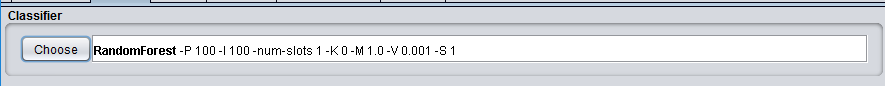
\includegraphics[width=1\linewidth]{images/algorithme.PNG}
\end{center}
\caption{Choix de l'algorithme de classification}
\label{fig:15}
\end{figure}

Tous les algorithmes présentés dans la section "Algorithme de classification"  (Random forest, Decision tree, Support vector machines, neural network, KNN, Naive Bayes) sont disponibles dans WEKA en cliquant sur le bouton "choose". L'objectif c'est de les pouvoir exécuter et récupérer leurs performances.

\subsubsection{Forêt aléatoire (Random forest) :}

Après l'exécution de l'algorithme Random forest sur notre échantillon de données on a eu les résultats montrés dans la figure ci-dessous, avec une précision de 27\%.

\begin{figure}[H]
\begin{center}
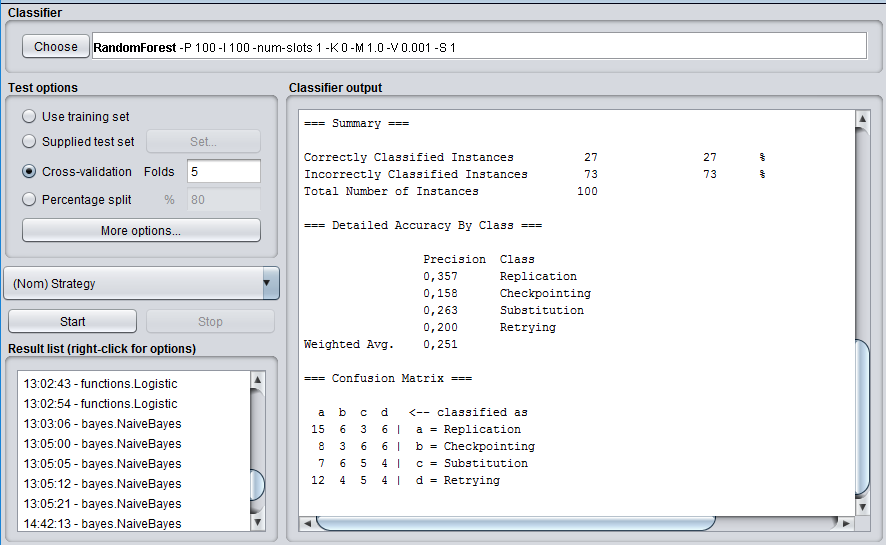
\includegraphics[width=0.8\linewidth]{images/perfRF.PNG}
\end{center}
\caption{Performance de Random Forest}
\label{fig:16}
\end{figure}


\subsubsection{L'arbre de décision (Decision Tree) :}

L'algorithme Decision Tree, a donné 27\% de précision après son exécution.

\begin{figure}[H]
\begin{center}
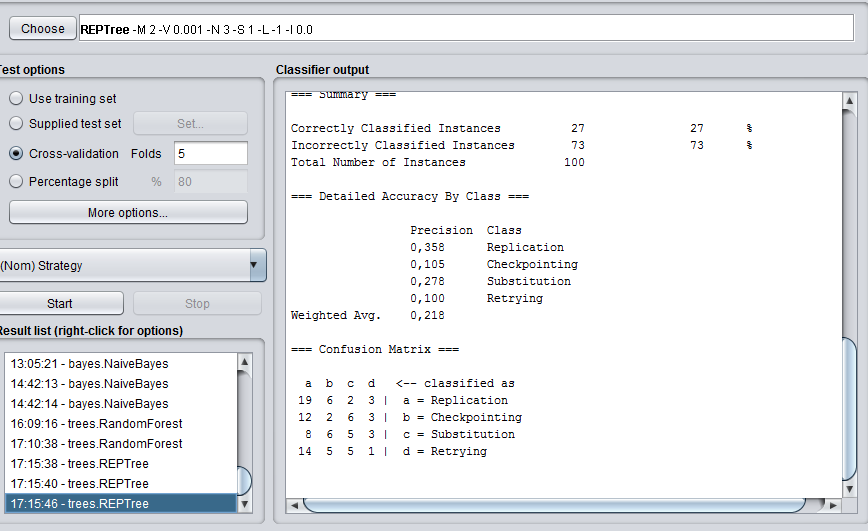
\includegraphics[width=0.8\linewidth]{images/perfDecTree.PNG}
\end{center}
\caption{Performance de Decision Tree}
\label{fig:17}
\end{figure}


\subsubsection{Machine à vecteurs de support (Support vector Machine) :}

Après l'exécution de l'algorithme Support sur notre échantillon de données on a eu un résultat de 31\% de précision.

\begin{figure}[H]
\begin{center}
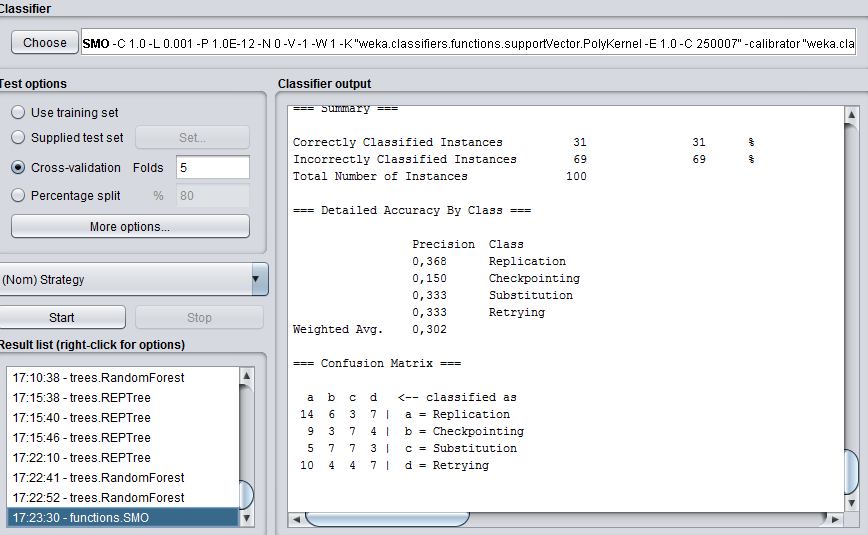
\includegraphics[width=0.8\linewidth]{images/perfSMO.PNG}
\end{center}
\caption{Performance de Support vector Machine }
\label{fig:18}
\end{figure}

\subsubsection{Réseau de neurones (Neural Network) :}

Après l'exécution de l'algorithme Neural Network sur notre échantillon de données on a eu les résultats montrés dans la figure ci-dessous, avec une précision de 30\%.

\begin{figure}[H]
\begin{center}
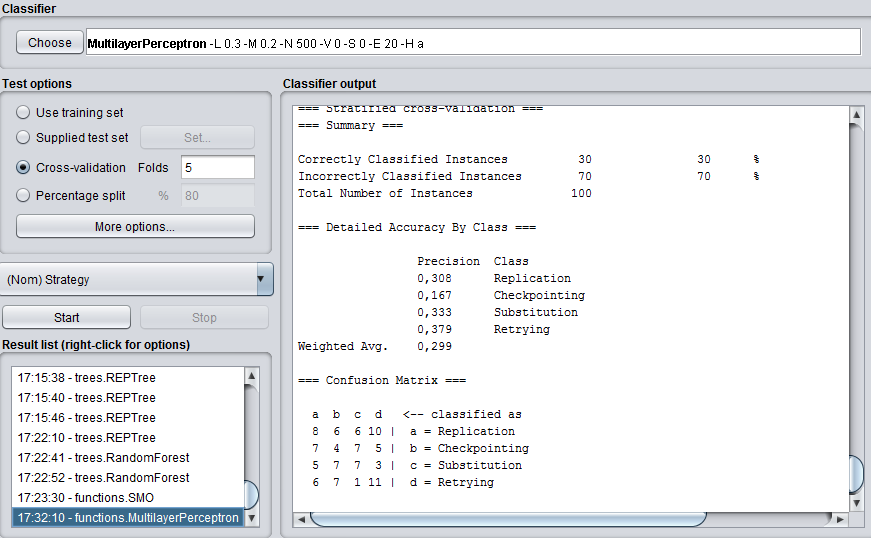
\includegraphics[width=0.8\linewidth]{images/perfNN.PNG}
\end{center}
\caption{Performance de Neural Network}
\label{fig:19}
\end{figure}

\subsubsection{Les k plus proches voisins (K-Nearest Neighbors KNN)}
Après l'exécution de l'algorithme KNN sur notre échantillon de données on a eu un résultat de 22\% de précision.

\begin{figure}[H]
\begin{center}
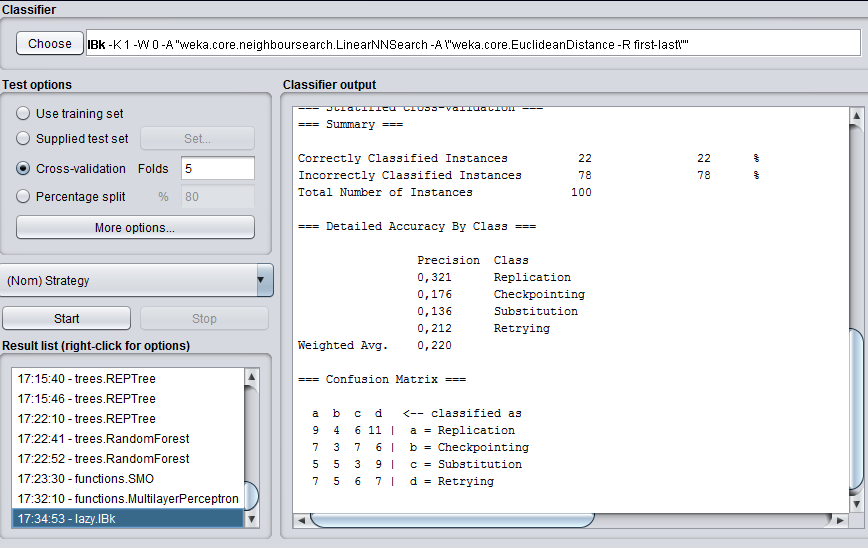
\includegraphics[width=0.8\linewidth]{images/perfKNN.PNG}
\end{center}
\caption{Performance de KNN}
\label{fig:20}
\end{figure}

\subsubsection{Naive Bayes}

L'algorithme Decision Tree, a donné 32\% de précision après son exécution.

\begin{figure}[H]
\begin{center}
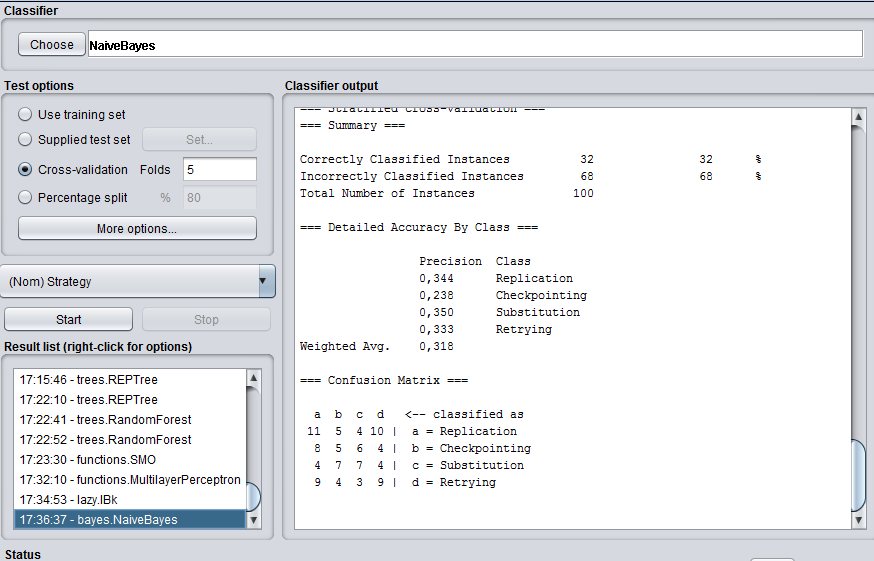
\includegraphics[width=0.8\linewidth]{images/perfNB.PNG}
\end{center}
\caption{Performance de Naive Bayes}
\label{fig:21}
\end{figure}

Résultat : 

D'après les résultats obtenus après l'exécution de chaque algorithme on a résumé les précisions dans le tableau suivant : 

\begin{figure}[H]
\begin{center}
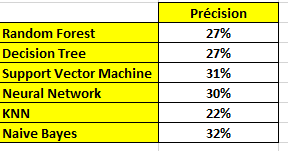
\includegraphics[width=0.7\linewidth]{images/stat.PNG}
\end{center}
\caption{Tableau concluant la précision des algorithme}
\label{fig:22}
\end{figure}

Les résultats montrent que les modèles les plus précis sont ceux obtenus par l'algorithme de Naive Bayes et  de Support Vector Machine avec une précision de 32\% et 31\%.

Cela reste une hypothèse comme cité au par avant car les données sur lesquelles on se base sont des données temporaires, qui sont générées d'une manière aléatoire a priori pour décrire le processus de prédiction de la stratégie de récupération. 


\chapter{Conclusion}

\section{Conclusion générale}

Ce mémoire avait pour ambition de proposer comment peut on exploité une base d'informations générée pour décider une stratégie de récupération, dans le cas d'une panne sur les services composites. 

Pour répondre a cette question, nous avons proposé une approche prédictive du mécanisme de récupération des services Web composites en cas de panne, notre étude se base sur l'approche auto-corrective (self healing) de l'exécution des services composites, qui a proposé un exécuteur basé sur des agents à base de connaissances capables d'analyser l'exécution d'un service composite, et de déduire de nouvelles informations à partir de cette analyse, ces informations ont un rôle crucial dans le processus de prise de décision lors de l'exécution, et c'est au niveau de cette phase qu'intervient notre contribution présentée dans ce mémoire, nous avons exploité toutes ces informations pour en pouvoir construire un modèle de classement par mécanisme de récupération, afin de prédire en cas de panne la stratégie de récupération qui vas être mise en pratique. 

Ainsi nous avons mis oeuvre des algorithmes de l'auto apprentissage (Machine Learning) pour la prise de décision d'une manière dynamique et automatique sans avoir besoin d'intervention humaine.

La réalisation du présent mémoire m'a permet de rentré dans le monde de l'intelligence artificielle, en découvrant les différents domaines de problématiques de l'apprentissage automatique, ainsi que les algorithmes spécifiques à chaque famille de problématiques, sans oublier les méthodes statistiques d'évaluation des performances des modèles obtenus.

\section{Limites et Perspective }

La limite la plus importante de ce mémoire se situe au niveau de la phase de traitement et d'analyse des données pour l'apprentissage automatique.
L'équipe des chercheurs responsables du projet de l'exécuteur auto-corrective, avec lesquels on travaille, et sur leurs données générées qu'on se base pour l'auto apprentissage, ont eu des problèmes au niveau de stockage du coups ils ont perdu l'ensemble des données concernées.

Donc la réalisation a été basée sur des données qui sont générées d'une manières aléatoire, pour bien décrire le processus suivis de la mis en oeuvre de l'apprentissage automatique a travers les outils déployés (Pentaho/WEKA).
Mais le résultat final de l'analyse qui consiste le choix de l'algorithme le plus précis pour prédire la stratégie de récupération reste une hypothèse ouverte puisque nos données sont aléatoire.
 
Nos perspectives sont sur le même niveau que nos limites, on envisage obtenir des données qui sont réelles générées par l'exécuteur d'auto-corrective pour pouvoir sélectionnée un modèle de prédiction définitif, sur lequel on peux se baser pour prendre les décisions de choix du mécanisme de récupération en cas de panne des services Web composites.




\appendix


\bibliographystyle{authoryear-fr}
\bibliography{reference}


\end{document}